\documentclass[16pt]{beamer}
\usetheme{Ilmenau}
\usecolortheme{beaver}
\usepackage[utf8]{inputenc}
\usepackage[german]{babel}
\usepackage{amsmath}
\usepackage{amsfonts}
\usepackage{amssymb}
\usepackage{graphicx}
\author{Jeremias Eppler, Jochen Morent, Georgi Georgiev}
\title{Projektcontrolling - Lindale }
\begin{document}
\maketitle

\begin{frame}{Ablauf des Projektcontrollingprozess}
\begin{itemize}
  \item Erfassung von Ist-Daten und 
  \item Durchführung des Soll-Ist-Vergleich
  \item Steuernde Maßnahmen erarbeiten
  \item Neuplanung: Updating der Projektpläne
  \item Erstellung von Projektfortschrittsberichten, Project Score Card
  \item Projektdurchführung fortsetzen bis zum nächsten Projektcontrolling
\end{itemize}
\end{frame}

\begin{frame}{Projektcontrolling-Zyklus}
\begin{figure}
\includegraphics[width=0.6\textwidth, height=0.6\textheight, keepaspectratio]{image/projekcontrolling-zyklus}
\caption{Projektcontrolling-Zyklus}
\end{figure}
\end{frame}

\begin{frame}{Wozu braucht man das Projektcontrolling?}
\begin{itemize}
  \item Der Projektcontrollingprozess passt die Planung der eigendynamik des Projekts an
  \item Alle Projektbeteiligten können über den aktuellen Stand des Projektes informiert werden
  \item Möglichkeit bei starken Abweichungen zu korrigieren
  \item Das Projekt wird kontrolliert und gesteuert $\rightarrow$ effiziente Zielerreichung
\end{itemize}
\end{frame}

\begin{frame}{Wozu braucht man das Projektcontrolling?}
\begin{itemize}
  \item Der Projektcontrollingprozess passt die Planung der eigendynamik des Projektes an
  \item Alle Projektbeteiligten können über den aktuellen Stand des Projektes informiert werden
  \item Möglichkeit bei starken Abweichungen Gegenmaßnahmen zu erreichen
  \item Das Projekt wird kontrolliert und gesteuert $\rightarrow$ effiziente Zielerreichung
\end{itemize}
\end{frame}

\begin{frame}{Projektcontrolling innerhalb von Lindale}
\begin{itemize}
  \item Eingesetze Methoden:
  \begin{itemize}
    \item Projektfortschrittsbericht
    \item Projekt Score Card
  \end{itemize}
  \item Updaten der Projektplänen $\rightarrow$ z. B. verzug beim Modellieren des Projektes
  \item Wöchentliches Teammeeting bei dem bereits über die Entwicklung der vergangenen Woche reflektiert wird 
\end{itemize}
\end{frame}

\begin{frame}{Projekt Score Card}
\begin{figure}
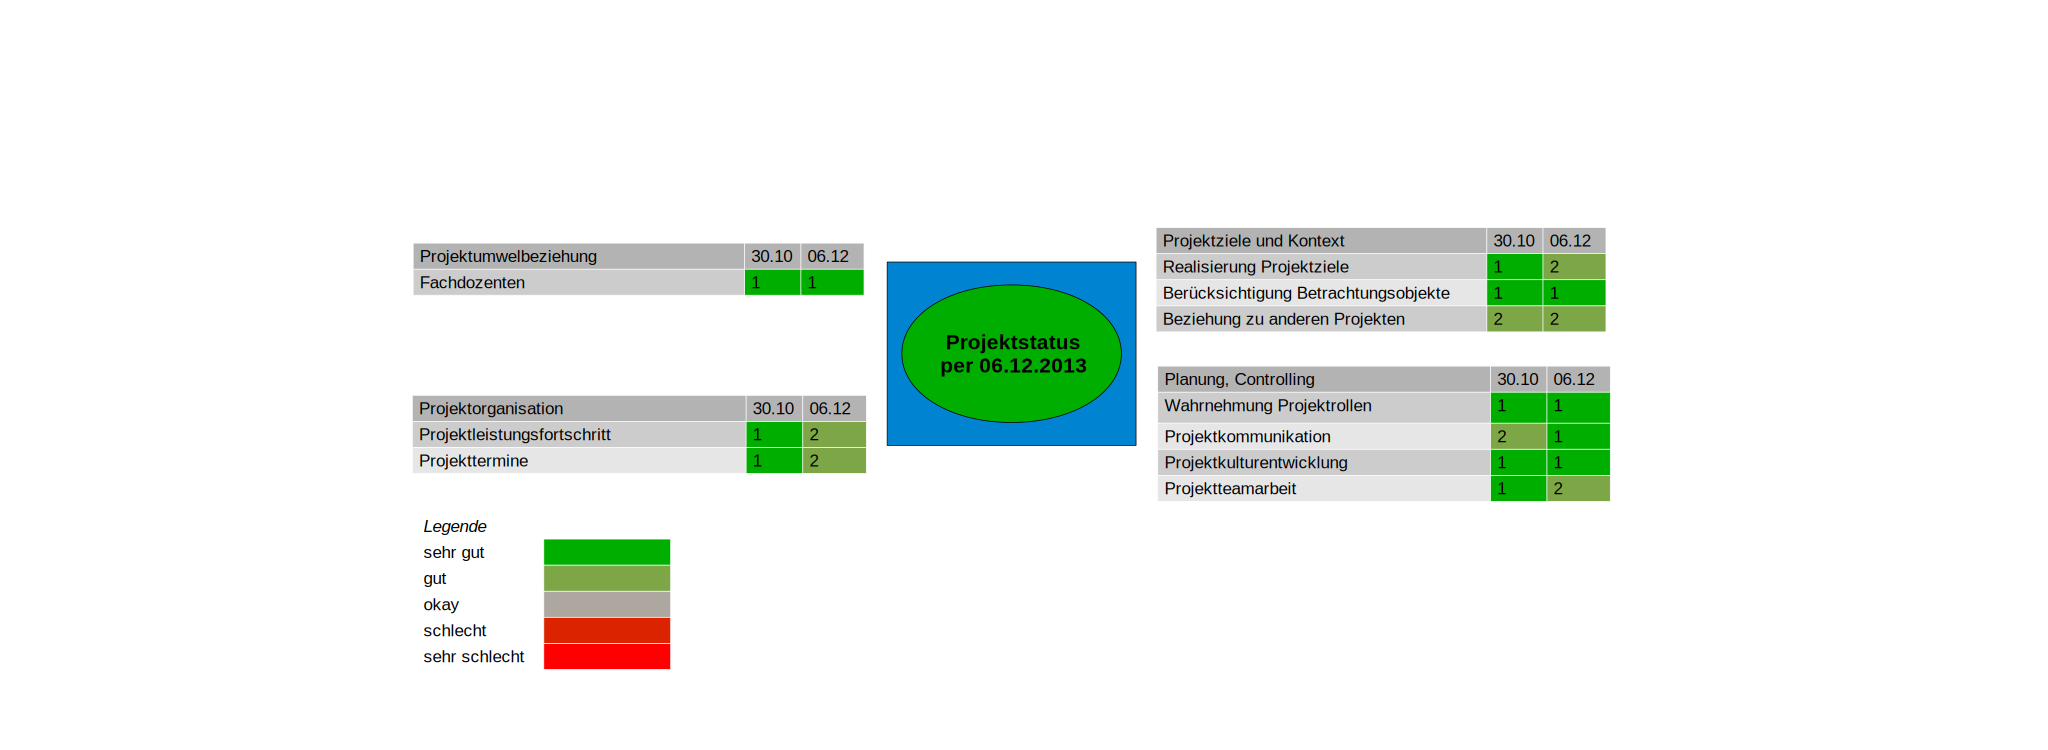
\includegraphics[width=\textwidth, height=\textheight, keepaspectratio]{image/projekt-score-card}
\caption{Projekt Score Card für Lindale}
\end{figure}
\end{frame}

\end{document}